\chapter{Super-Resolução Pós-Inversão Sísmica}
\label{cap:3modeloHibrido}

Neste Capítulo é apresentada a metodologia discutida neste trabalho.
São apresentadas as estratégias iniciais de aplicação do modelo convolucional,
os resultados preliminare e o cronograma de atividades.

\section{Modelo de Super-Resolução}

No capítulo anterior foi apresentado o método de inversão acústica que
representa o estado da arte no cálculo do máximo \textit{a posteriori} (MAP) para determinar o
resultado mais provável \citep{Buland01012003, leandroGRSL}. Foram apresentados os trabalhos relacionados
com o desenvolvimento de modelos de redes neurais convolucionais para tratar problemas de
super-resolução \citep{Oord16,He2016,DahlNS17}. 
 
A presente proposta tem como objetivo o emprego de um modelo de rede neural convolucional
para aumentar a resolução das imagens de impedância acústica
resultantes do processo de inversão sísmica. Com esta abordagem se espera obter um ganho
quantitativo, através da inserção de altas frequências no espectro de frequência da
propriedade, e qualitativo, com a entrega de imagens com maior definição entre camadas.
Além disto, por se tratar de um problema de inversão, um estudo de incerteza sobre os
resultados das redes convolucionais será realizado sobre os resultados.

O modelo apresentado por \cite{DahlNS17} admite que cada \textit{pixel} pode assumir valores discretos entre
$0$ e $255$, e funciona como uma rede classificadora. Para ser aplicado sobre dados geoestatísticos o modelo
necessita ser ajustado para ser capaz de realizar regressão
diretamente sobre os valores de impedância, ou para impedância normalizada no intervalo real
$[-1,+1]$. Com isto, se espera abandonar a discretização dos valores de impedância utilizadas
nos experimentos iniciais, uma vez que esta medida causou a perda de informação. 
Embora os autores pontuem as dificuldades para implementação de um modelo regressivo,
se acredita ser razoável realizar uma nova investigação sobre a implementação de um
modelo convolucional que realize a pervisão para valores contínuos. Esta adaptação
passa pela substituição da função de \textit{softmax} e modificação da função de custo.

Para realizar a inversão acústica é necessário ter disponível a sísmica, a \textit{wavelet}
e o modelo de baixa frequência para impedância acústica ($<8Hz$) %(Equação \ref{eqn:mapSolution}).
O fluxo de trabalho segue as etapas listadas:
 
\begin{enumerate}
  \item Parametrização do método de inversão acústica com a sísmica, a \textit{wavelet} e o modelo de baixa frequência.
  \item Geração das imagens de baixa resolução
  \item Normalização das imagens de impedância para escala de cinza.
  \item Divisão do conjunto de dados entre conjunto de treinamento e conjunto de teste.
  \item Treinamento do modelo de rede convolucional com os pares de imagens de treinamento.
  \item Amostragem das imagens de alta resolução a partir das imagens de teste de baixa resolução.
  \item Comparação entre as imagens obtidas da rede e a imagem real.
  \item Recuperação dos valores de impedância das imagens de alta resolução obtidas.
\end{enumerate}

A rede convolucional é um modelo cujo treinamento é supervisionado, de modo que,
para otimizar seus parâmetros, é necessário dispor dos pares de imagens de alta
e baixa resolução. Uma vez a rede convolucional treinada, é possível aumentar a
resolução de imagens provenientes de outros cenários da inversão acústica.

\section{Resultados Preliminares}
Os primeiros experimentos exploraram o potencial do modelo de rede convolucional que representa
o estado da arte em super-resolução. Este modelo foi adaptado para realizara super-resolução
sobre dois conjuntos de dados sintéticos. O primeiro conjunto de dados representa uma estrutura
geológica em formato de cunha envolto de uma segunda estrutura.
O segundo conjunto consiste em um cubo de impedâncias sintéticas usadas para realizar a inversão
sísmica para a própria impedância.
Em ambos os casos as imagens foram discretizadas de modo que cada \textit{pixel} $I_{i,j}$ assume 
valores entre $0$ e $255$, com aplicação da Equação \ref{eqn:norm_im}:

\begin{equation}
 K_{(i,j)} = \floor*{\big( \frac{256*(I_{i,j} - min(I))}{max(I)} \big)},
\label{eqn:norm_im}
 \end{equation}

onde $max(I)$ é o \textit{pixel} de maior intensidade e $min(I)$ é o \textit{pixel} de menor intensidade
na imagem $I$. Os valores de maior e menor intensidade de cada \textit{pixel} foi armazenado, de modo que é
possível recuperar os valores de impedância das imagens de alta resolução obtidas pela rede
se todos os valores forem armazenados para posterior aplicação na função inversa. Entetando,
a função de arredondamento aplicada gera uma perda de informação.

\subsection{Caso sintético: Cunha}
Neste caso, foram geradas $640$ imagens de tamanho $32$ x $32$ de uma estrutura geológica em forma
de cunha, perfazendo um total de $20$ grupos de treinamento. Adicionalmente, foram geradas $32$
novas imagens para teste da rede. As estruturas criadas correspondem a valores de impedância
acústica na profundidade e representam um conjunto de dados simples, pois os valores
de impedância possuem... 

Para gerar o conjunto de imagens de baixa resolução, as imagens foram filtradas por meio de filtro
passa baixa, com frequência de corte em $4Hz$. A Figura \ref{fig:cunhas} apresenta um conjunto exemplo
usado no treinamento da rede convolucional para o caso em questão. A Figura \ref{fig:cunhahr} exibe
a cunha sintética em alta resolução e a Figura \ref{fig:cunhalr} apresenta a mesma cunha filtrada.
\begin{figure}[htp]
\centering
\begin{subfigure}{.8\textwidth}
  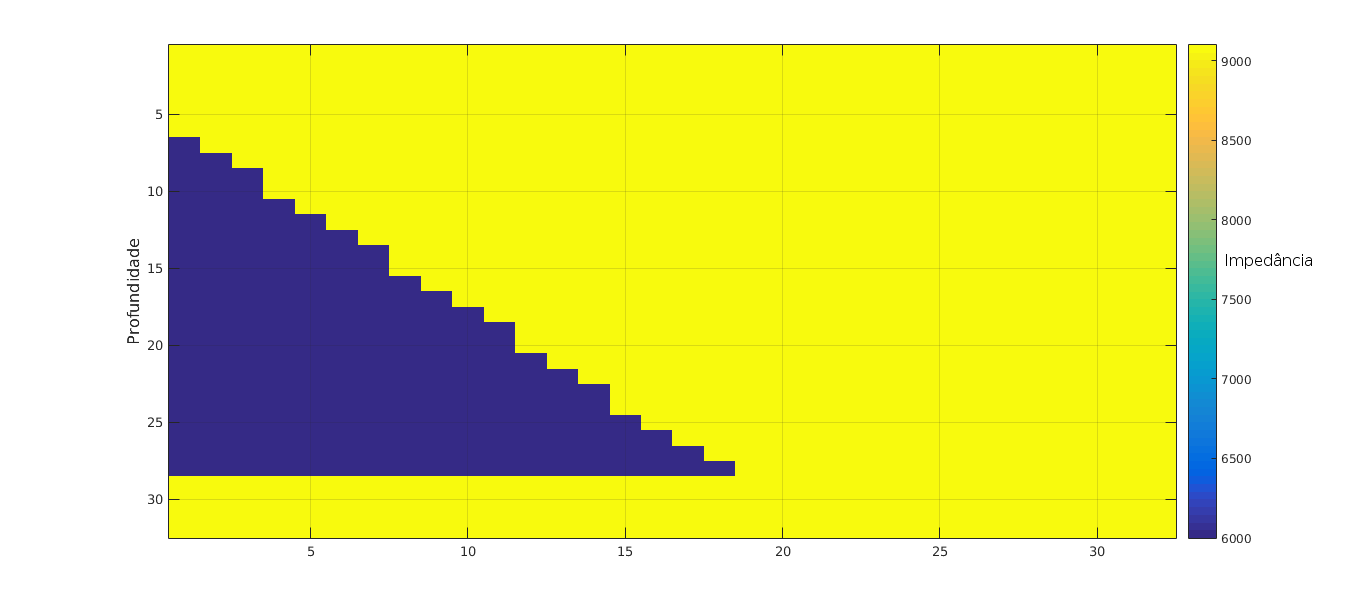
\includegraphics[width=.9\linewidth]{fig/cunha_hr}
  \caption{Cunha em alta resolução.}
  \label{fig:cunhahr}
\end{subfigure}
\begin{subfigure}{.8\textwidth}
  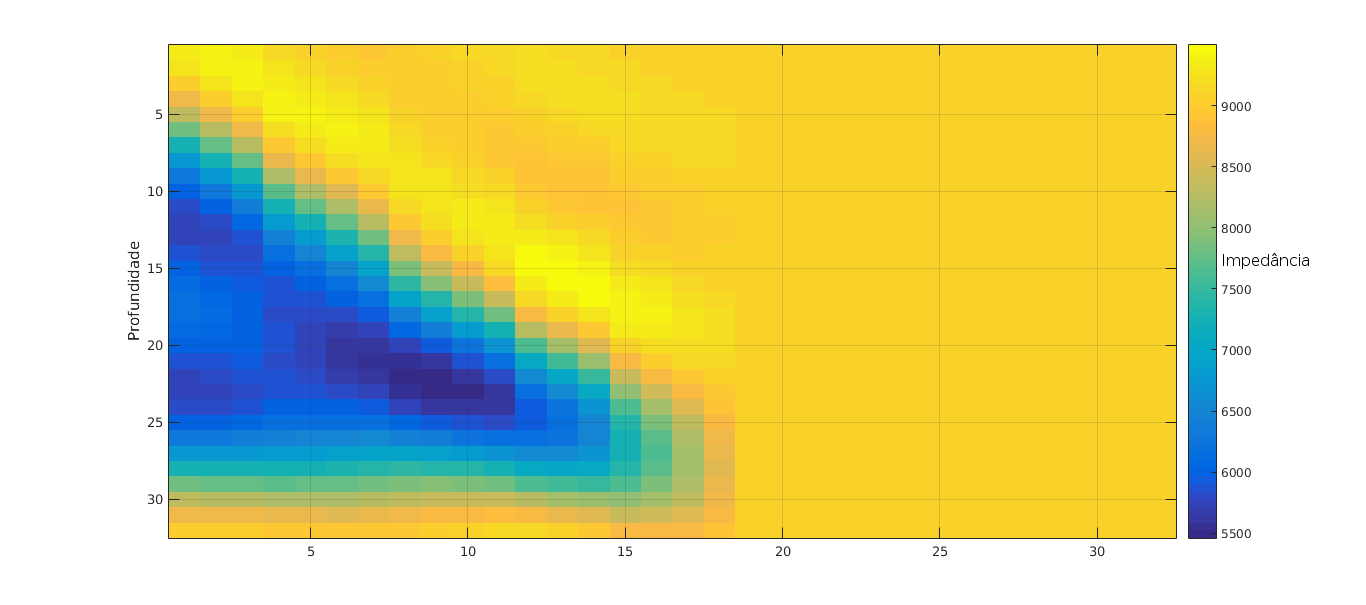
\includegraphics[width=.9\linewidth]{fig/cunha_lr}
  \caption{Cunha Filtrada.}
  \label{fig:cunhalr}
\end{subfigure}%
\caption{Exemplo de um conjunto de treinamento da rede convolucional.}
\label{fig:cunhas}
\end{figure}

Nas Figuras \ref{fig:cunha_pixel_lr}, \ref{fig:cunha_pixel_hr} e \ref{fig:result_cunha_pixel} é possível comparar
o resultado da super-resolução com a imagem sintética da cunha. Na Figura \ref{fig:cunha_pixel_lr} são apresentas as imagens filtradas em
baixa resolução, na Figura \ref{fig:cunha_pixel_hr} são apresentadas as imagens de referência em alta resolução e na 
Figura \ref{fig:result_cunha_pixel} são apresentadas as imagens obtidas na saída da rede convolucional.
As imagens sintéticas e de baixa resolução são imagens de teste, de modo que não fizeram parte do conjunto de treinamento
da rede.

\begin{figure}[htp]
  \centering
  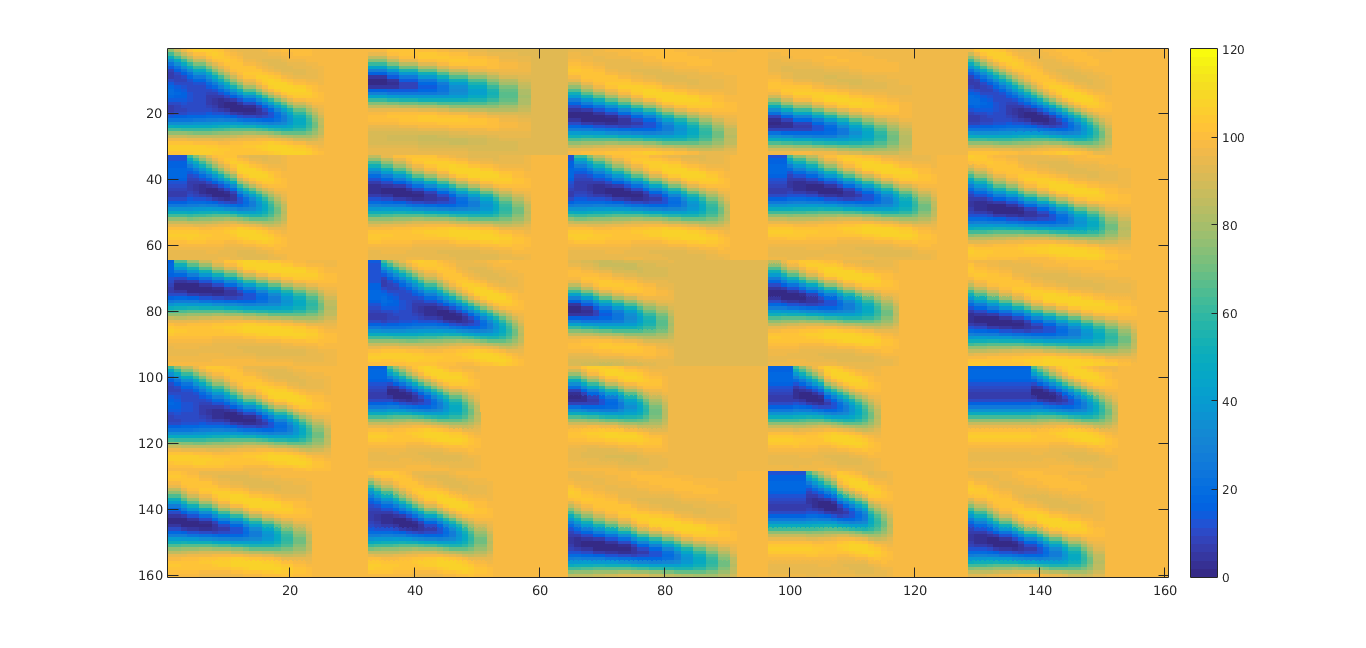
\includegraphics[width=.7\linewidth]{fig/cunha_pixel_lr}
  \caption{Imagens da cunha em baixa resolução.}
  \label{fig:cunha_pixel_lr}
\end{figure}

\begin{figure}
  \centering
  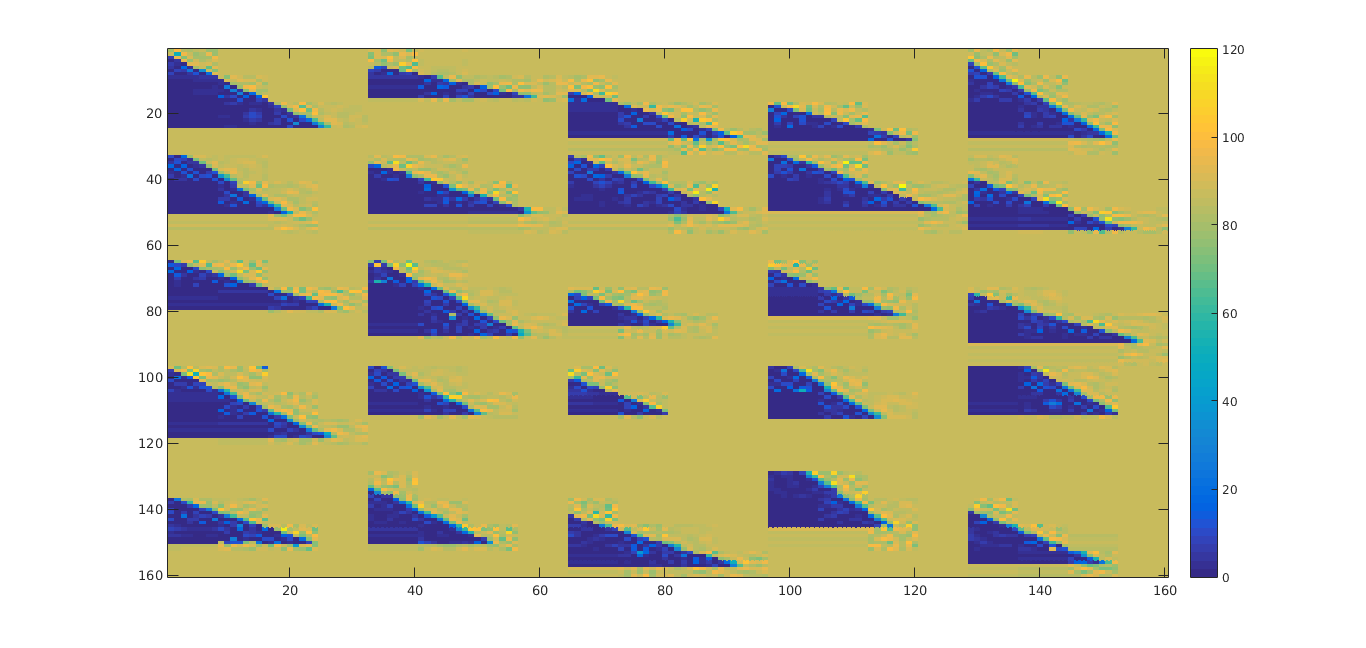
\includegraphics[width=.7\linewidth]{fig/result_cunha_pixel}
  \caption{Resultados da super-resolução.}
  \label{fig:result_cunha_pixel}
\end{figure}%

\begin{figure}
  \centering
  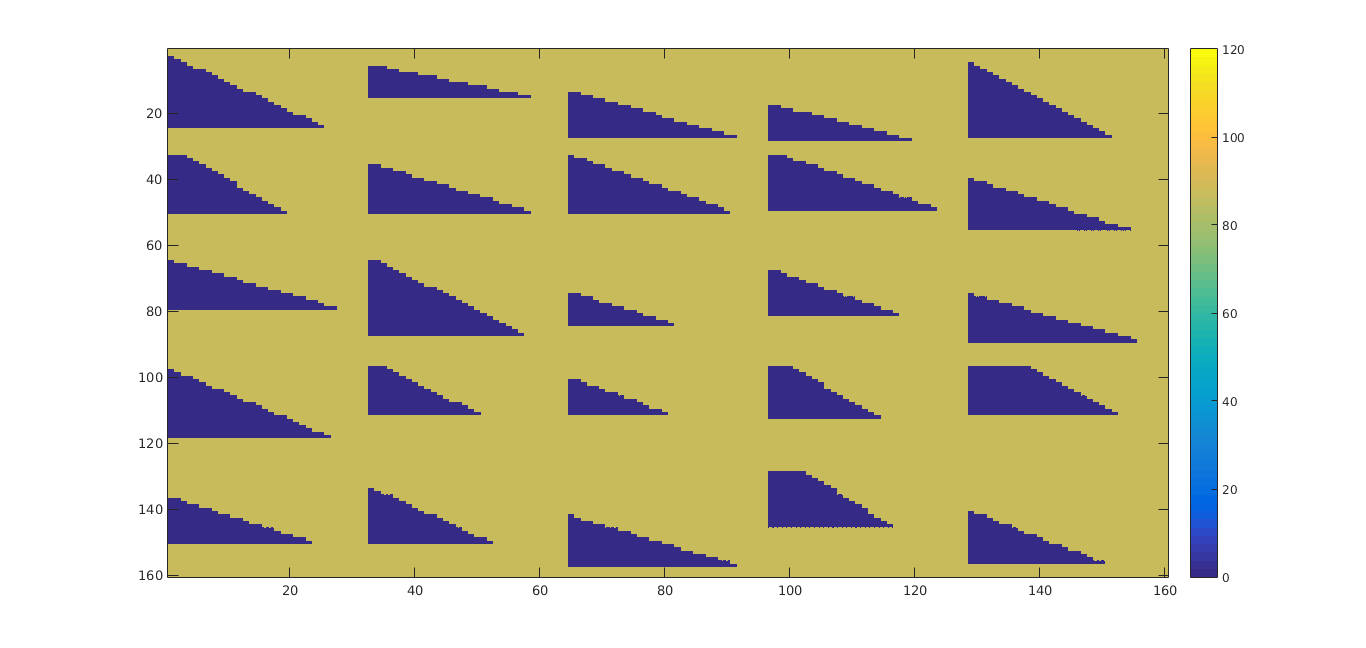
\includegraphics[width=.7\linewidth]{fig/cunha_pixel_hr}
  \caption{Imagens de cunhas em alta resolução.}
  \label{fig:cunha_pixel_hr}
\end{figure}

\subsection{Caso sintético: impedância Acústica}
Para realizar o segundo experimento foi utilizado um cubo sintético de impedância
acústica com $239$ imagens de dimensões $250$ x $199$. Do cubo de impedância foram calculados os
valores de refletividade. Uma \textit{wavelet}
sintética foi estimada e o cubo sísmico foi obtido por meio da
convolução entre a refletividade e a \textit{wavelet}. A este cubo sísmico foi adicionado ainda
$30\%$ de ruído. O cubo de impedância foi filtrado abaixo de $8Hz$ para obter o modelo de baixa frequência e
um ruído foi adicionado à sísmica. 
O método de inversão acústica por MAP foi parametrizado para disponibilizar imagens com nível elevado de ruído e baixa resolução.
Com isto é possível obter um resultado quantitativo e qualitativo da rede, ou seja, os resultados
obtidos podem ser avaliados sob a perspectiva da análise visual e do espectro de frequência.
Na figura \ref{fig:ipedances} estão ilustrados os exemplos de pares de imagens de alta e baixa resolução.
Por conta das limitações de memória de processamento, foi necessário realizar um recorte das imagens de impedância
obtidas da inversão. Para efeito de teste do modelo, foram utilizadas imagens com dimensões $32$ x $32$ do cubo de impedância.
O recorte realizado nas imagens compreendeu as regiões próximas do reservatório, como ilustrado nas Figuras \ref{fig:impedancehr}
e \ref{fig:impedancelr}.

\begin{figure}[htp]
\centering
\begin{subfigure}{.8\textwidth}
  \centering
  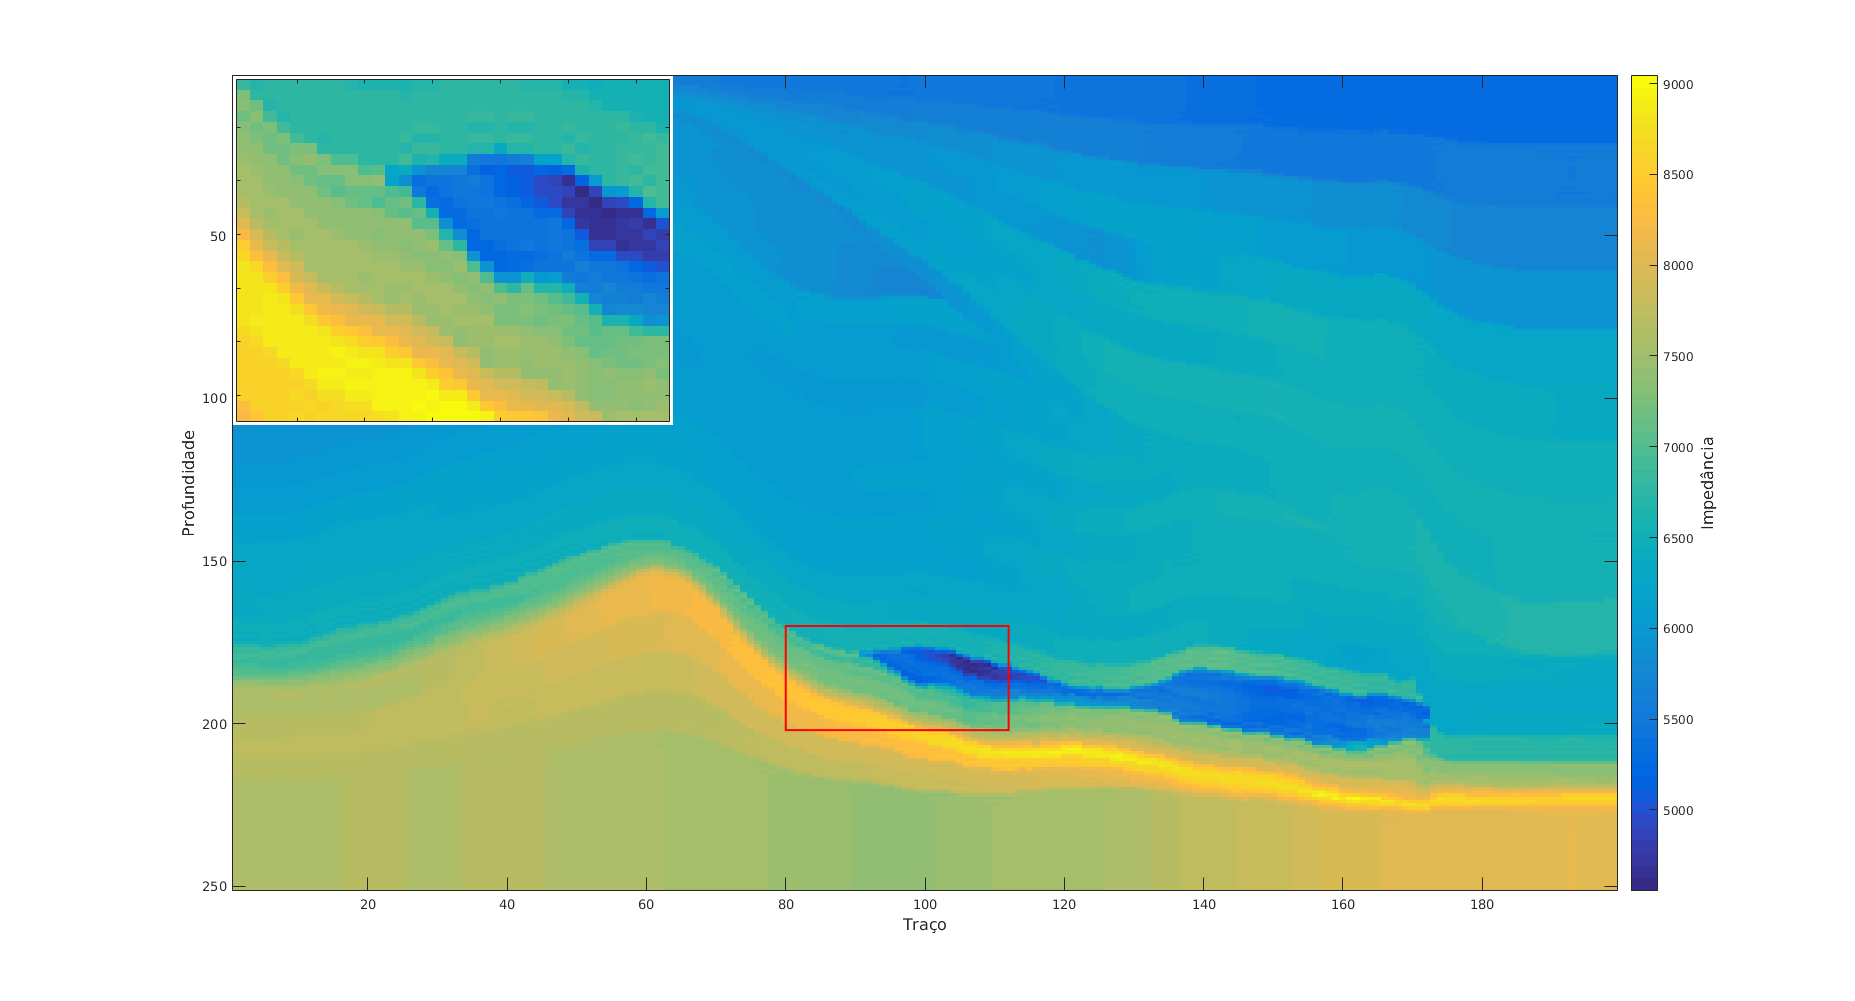
\includegraphics[width=.9\linewidth]{fig/impedance_mount}
  \caption{Seção do cubo de impedância sintética.}
  \label{fig:impedancehr}
\end{subfigure}
\begin{subfigure}{.8\textwidth}
  \centering
  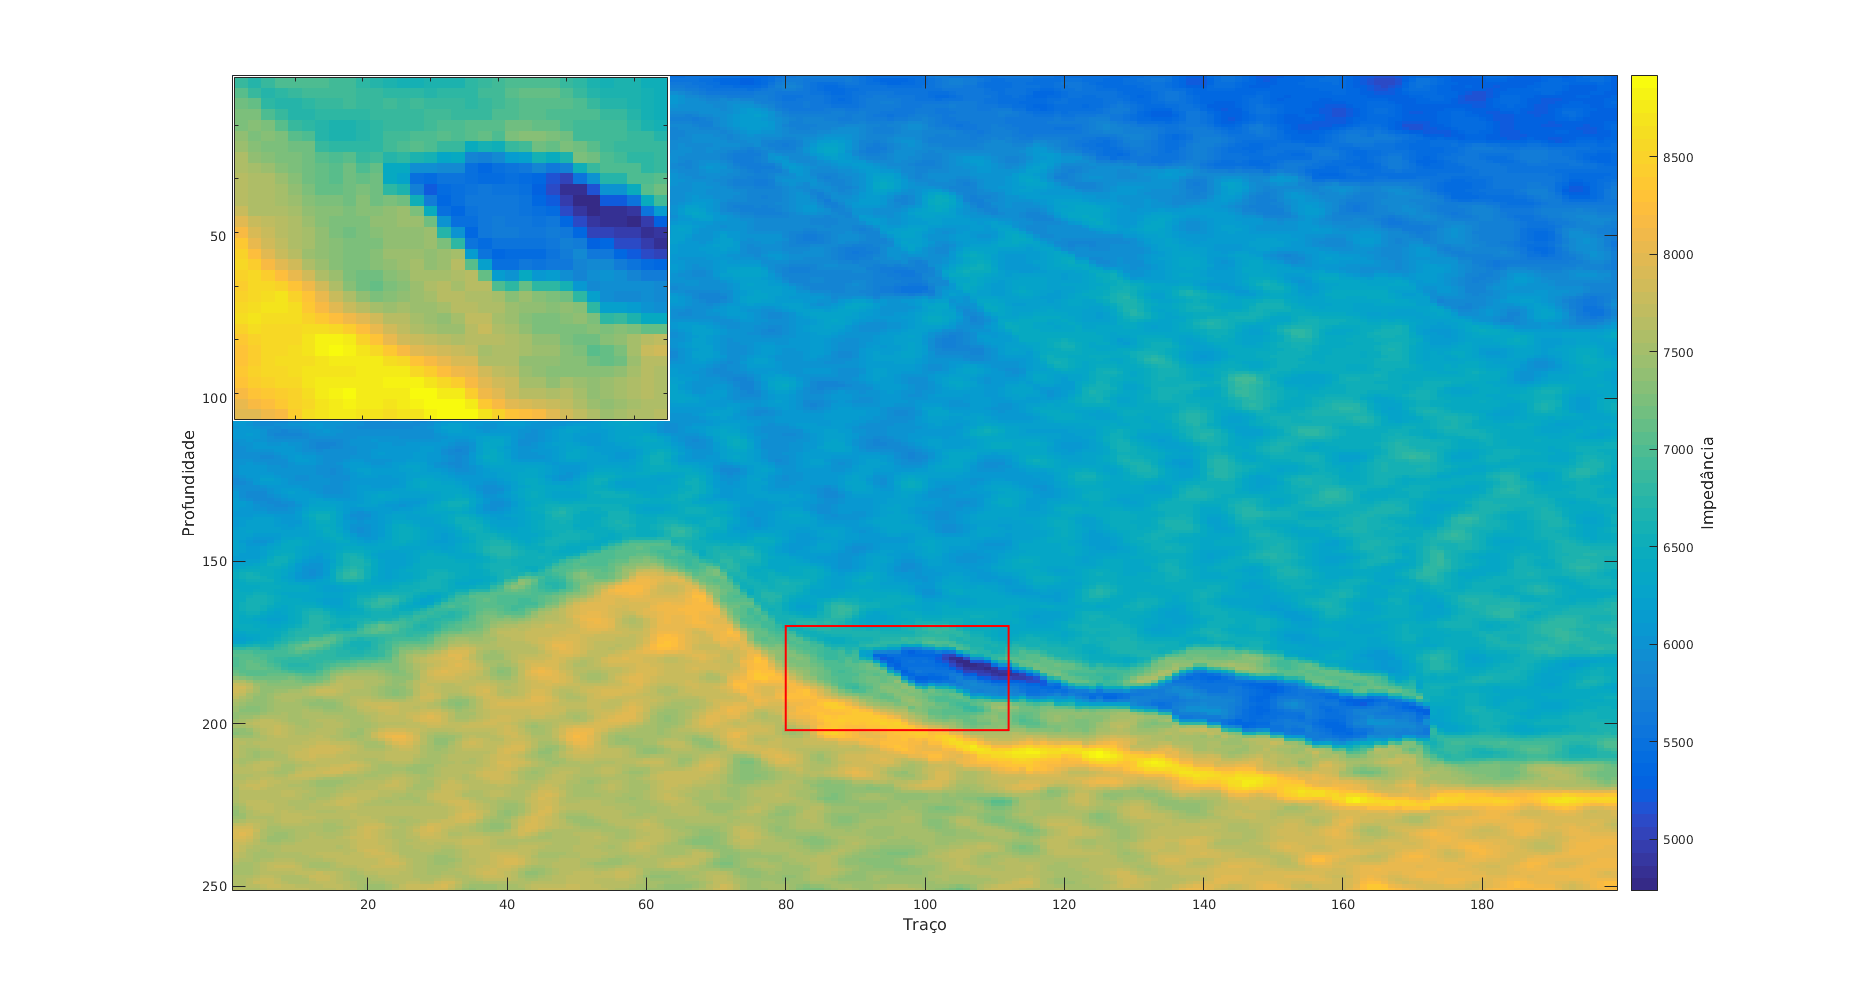
\includegraphics[width=.9\linewidth]{fig/inversion_mount}
  \caption{Resultado da inversão para a mesma seção do cubo.}
  \label{fig:impedancelr}
\end{subfigure}%
\caption{Seção do cubo de impedância da inversão MAP.}
\label{fig:ipedances}
\end{figure}

As redes convolucionais foram treinadas por 16 mil iterações e o modelo convergiu para erro (qual erro?) de ..
Nas Figuras \ref{} e \ref{} é possível notar que a rede é capaz de aumentar a resolução das imagens
da inversão sísmica, o ruido adicionado à sísmica e visível na inversão foi filtrado, e as camadas são mais evidentes.
A avaliação quantitativa é realizada utilizando uma métrica baseadad no Transformada Rápida de Fourier (FFT),
discutido na seção seguinte.


Uma estratégia para lidar com a limitação de memória de processamento é definir uma janela deslizante sobre as imagens, de
modo que cada imagem seja dividida em um novo conjuntos de treinamento composto por sub-imagens e a mesma rede pode
aprender com base nas sub-imagens. Um conjunto de sub-imagens pode ser usada para teste e, ao final, a imagem em tamanho
original é reconstruída a partir das subimagens de alta resolução obtidas pela rede.

\subsection{Transformada rápida de Fourier}

A Transformada Rápida de Fourier (FFT) foi utilizada como método de comparação entre as imagens calculadas pela rede
e as imagens de alta resolução de impedância esparsa. A métrica de similaridade entre as imagens é calculada usando a fórmula \ref{eq:fourier}, baseada
no espectro de frequência das imagens.
\begin{equation}
 C = \frac{ (\sum_{i=1}^{N}{F_{1i}F_{2i}} - N \bar{F}_1\bar{F}_2 )^2 }{ (\sum_{i=1}^{N}{|F_{1i}|^2} - N{\bar{F}^2}_1)( \sum_{i=1}^{N}{|F_{2i}|^2} - N{\bar{F}^2}_2 ) }
 \label{eq:fourier}
\end{equation}

Para cada frequência, um valor de intensidade é obtido das partes real e complexa da Transformada de Fourier.
Por conta da limitação de memória para processamento, foram utilizadas sub-imagens ($32$\textit{px} x $32$\textit{px}) das
imagens de impedância. $F_{1i}$ é o valor de intensidade do i-ésimo pixel da primeira imagem, enquanto $F_{2i}$
é o valor de intensidade do i-ésimo pixel da segunda imagem. $\bar{F}_1$ e $\bar{F}_2$ representam os valores
de frequência média de cada imagem. A métrica varia no intervalo de $0$ a $1$, sendo que, similaridade igual a $1$
representa a comparação entre imagens iguais.

A métrica $C$ foi calculada entre as imagens obtidas pela rede e as imagens de alta resolução de impedância esparsa, também, entre estas e
as imagens de MAP de impedância (baixa resolução). Com a utilização da métrica $C$, ficou evidente que as imagens em alta resolução obtidas com a rede apresentaram
maior similaridade com a imagem de impedância esparsa (alta resolução) e que, de fato a rede foi capaz de agregar elementos de
alta frequência à maioria das imagens de baixa resolução (MAP de impedância), em torno de $84\%$.

% 
% Experimentos realizados com o método para cálculo do MAP obtiveram resultados e
% tempo de execução comparáveis com métodos implementados na indústria
% \citep{leandroGRSL}. Apesar de resultar somente nas médias e variâncias, a
% parametrização e regularização utilizada na metodologia pode ajudar a restringir
% a amostragem, de forma a inserir informações da posterior e tornar a amostragem
% do SSD mais eficiente.
% 
% 
% Como a inversão GSI é fundamentada na Simulação Sequencial Direta, os resultados
% da primeira iteração da GSI são iguais aos resultados de uma SSD utilizando os
% mesmos parâmetros e dados de entrada. Desta forma é possível verificar a melhora
% na correlação da sísmica sintética com a sísmica original quando se utiliza o
% resultado do MAP como imagem secundária para SSD. Este experimento foi realizado
% e na primeira iteração do GSI a correlação das sísmicas sintética e original foi
% $0.45$ para a média de impedância, com a SSD utilizando o resultado do MAP como
% imagem secundária foi obtida uma correlação de $0.97$ para a média, foram
% utilizadas populações de $35$ amostras para cada método. Mesmo quando são
% executadas as iterações da GSI, a máxima correlação da média encontrada é $0.9$,
% tomando no mínimo 10 iterações para atingir este nível de qualidade.
% 
% Foram utilizados dados fornecidos pela PETROBRAS de um campo real para efetuar
% os testes. Os dados consistem de 4 poços que se encontram na posição dos traços
% 17, 210, 409 e 698, modelo de baixa frequência interpolado dos poços, horizontes
% e uma \textit{wavelet} extraída por um especialista da empresa. O parâmetro de
% distância de correlação da inversão por MAP foi utilizado $L=1.4$, a variância da sísmica
% foi estipulada como $0.4$ multiplicado pela variância média dos traços.
% Para a SSD foi utlizado um modelo de variograma horizontal omnidirecional
% esférico com alcance de $32$ traços, ou aproximadamente $800$ metros. Para o
% variograma vertical foi utilizando o mesmo modelo com o alcance de $2$ índices
% de tempo, correspondente a $8ms$.
% 
% O resultado da inversão MAP é demonstrado na Figura \ref{fig:mapResult}.
% A média das realizações amostradas pelo método proposto está na Figura
% \ref{fig:mapDSS}. Comparando com a Figura \ref{fig:dssresult}, a qual demonstra
% a média das realizações da primeira iteração da GSI, verifica-se que utilizar o
% resultado do MAP como imagem secundária traz a informação da sísmica nos pontos
% entre dos poços. Comparando a média da GSI após 10 iterações, na Figura
% \ref{fig:dss10result}, observa-se a semelhança dos resultados sem a necessidade
% de realizar as iterações. O método proposto demorou 52s para executar contra
% 487s para realizar as 10 iterações da GSI.
% 
% 
% 
% \begin{figure}[htp]
% \begin{center}
%   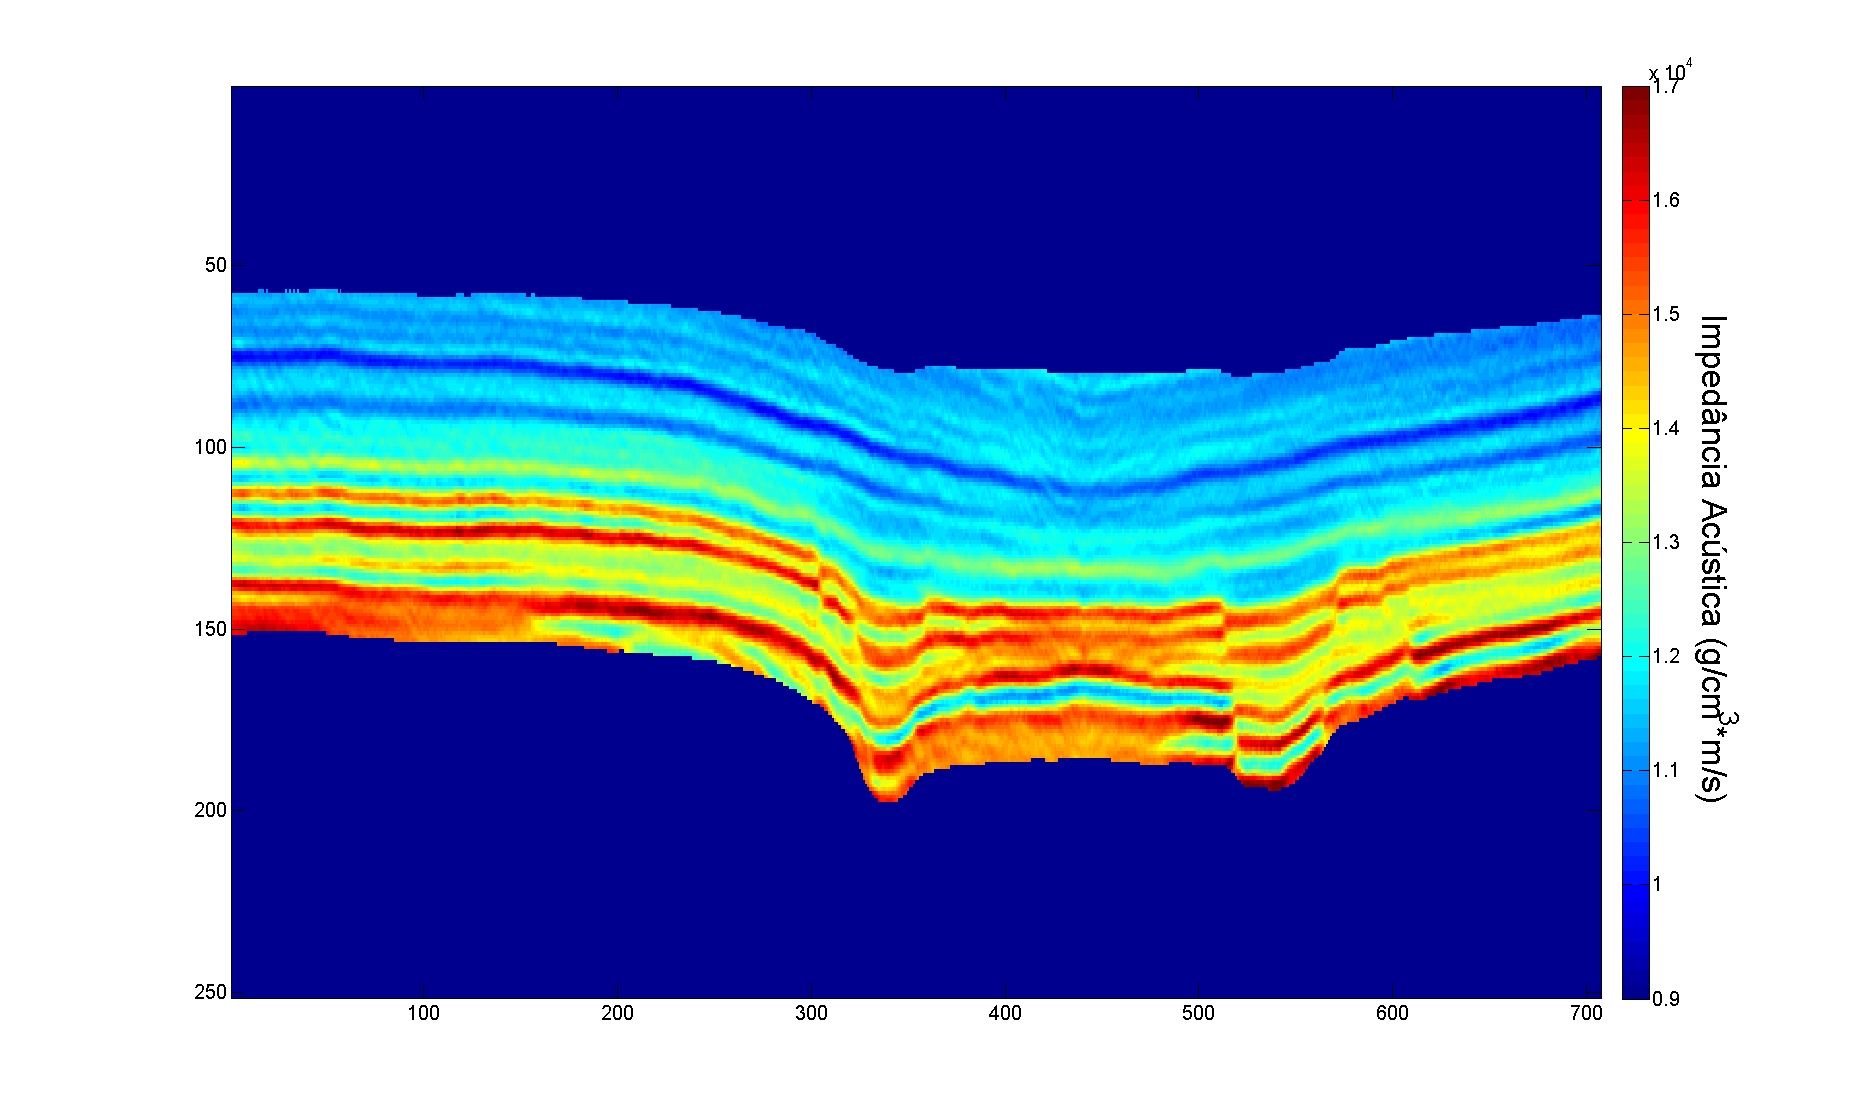
\includegraphics[width=\textwidth]{fig/map}
%   \caption{Resultado MAP utilizado como imagem secundária}
%   \label{fig:mapResult}
% \end{center}
% \end{figure}
% 
% 
% \begin{figure}[htp]
% \begin{center}
%   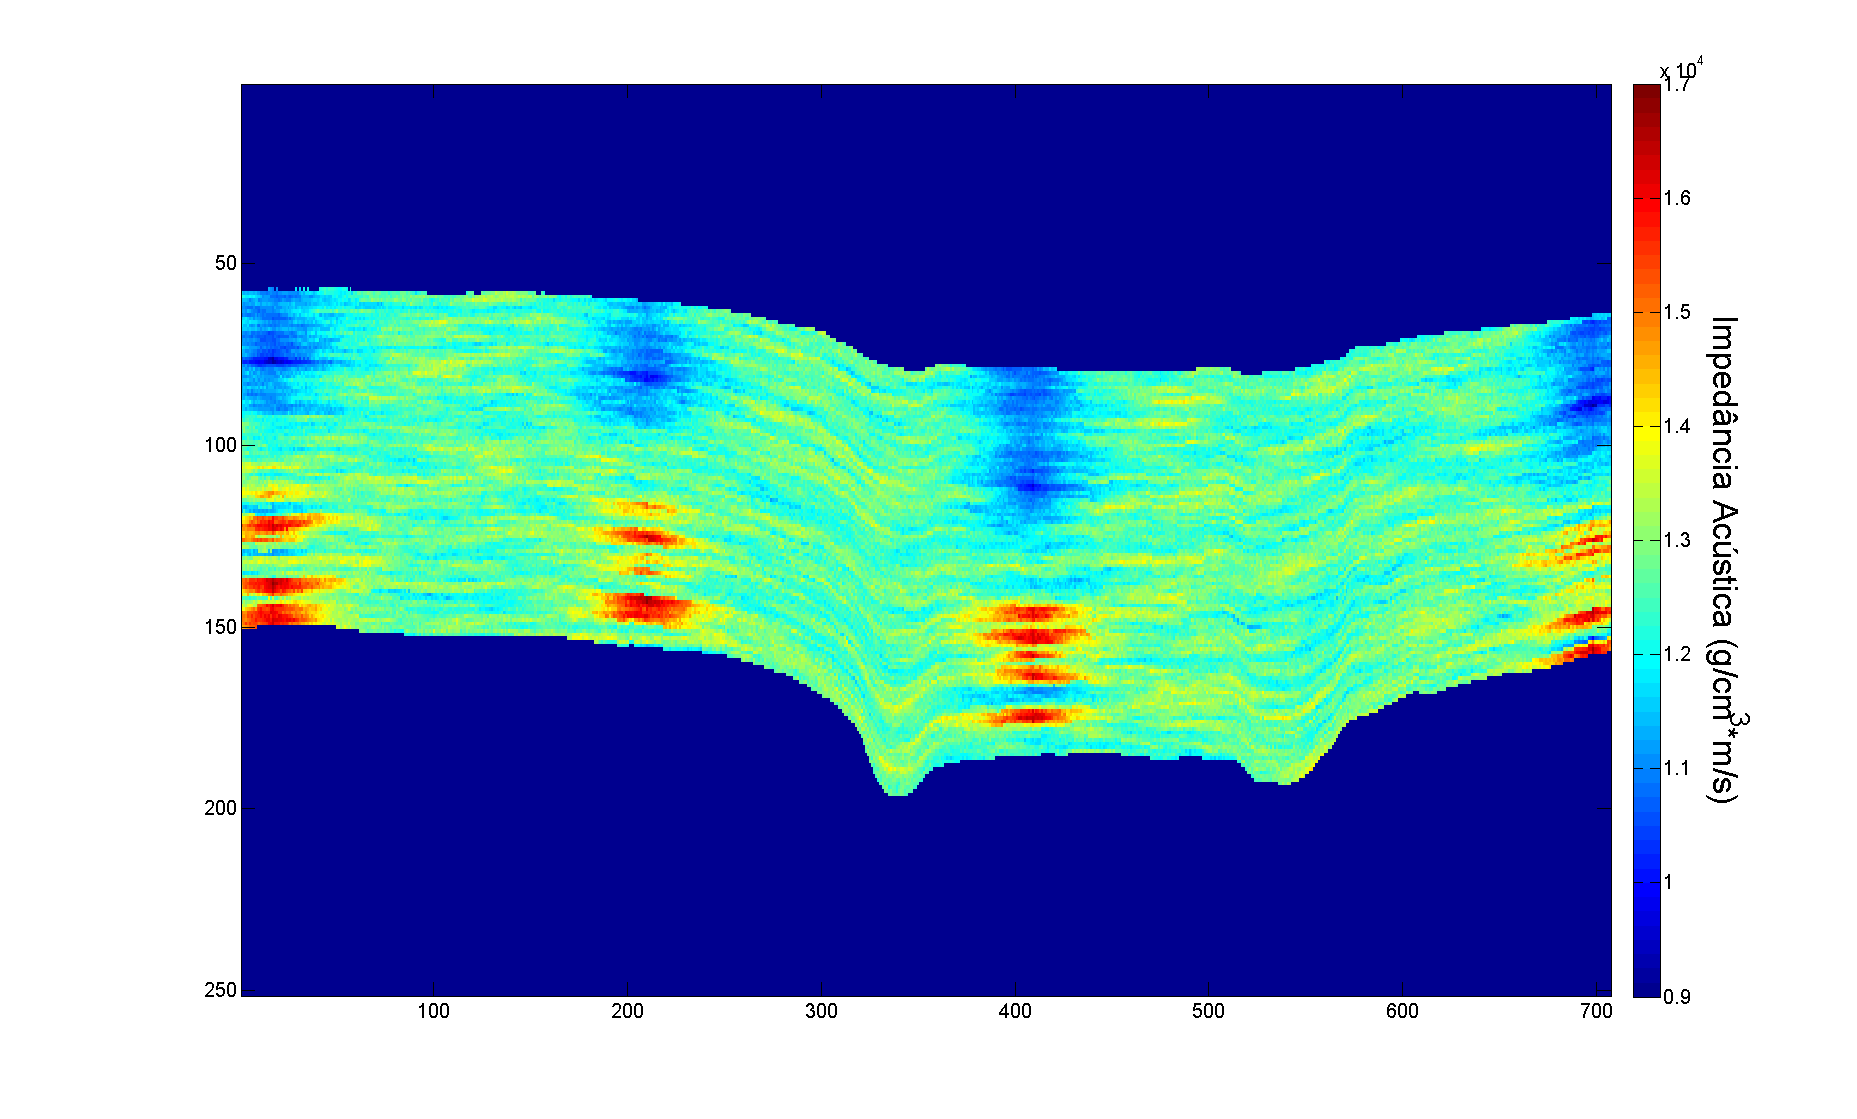
\includegraphics[width=\textwidth]{fig/dss1it-20realz}
%   \caption{Média das amostras da primeira iteração da GSI}
%   \label{fig:dssresult}
% \end{center}
% \end{figure}
% 
% \begin{figure}[htp]
% \begin{center}
%   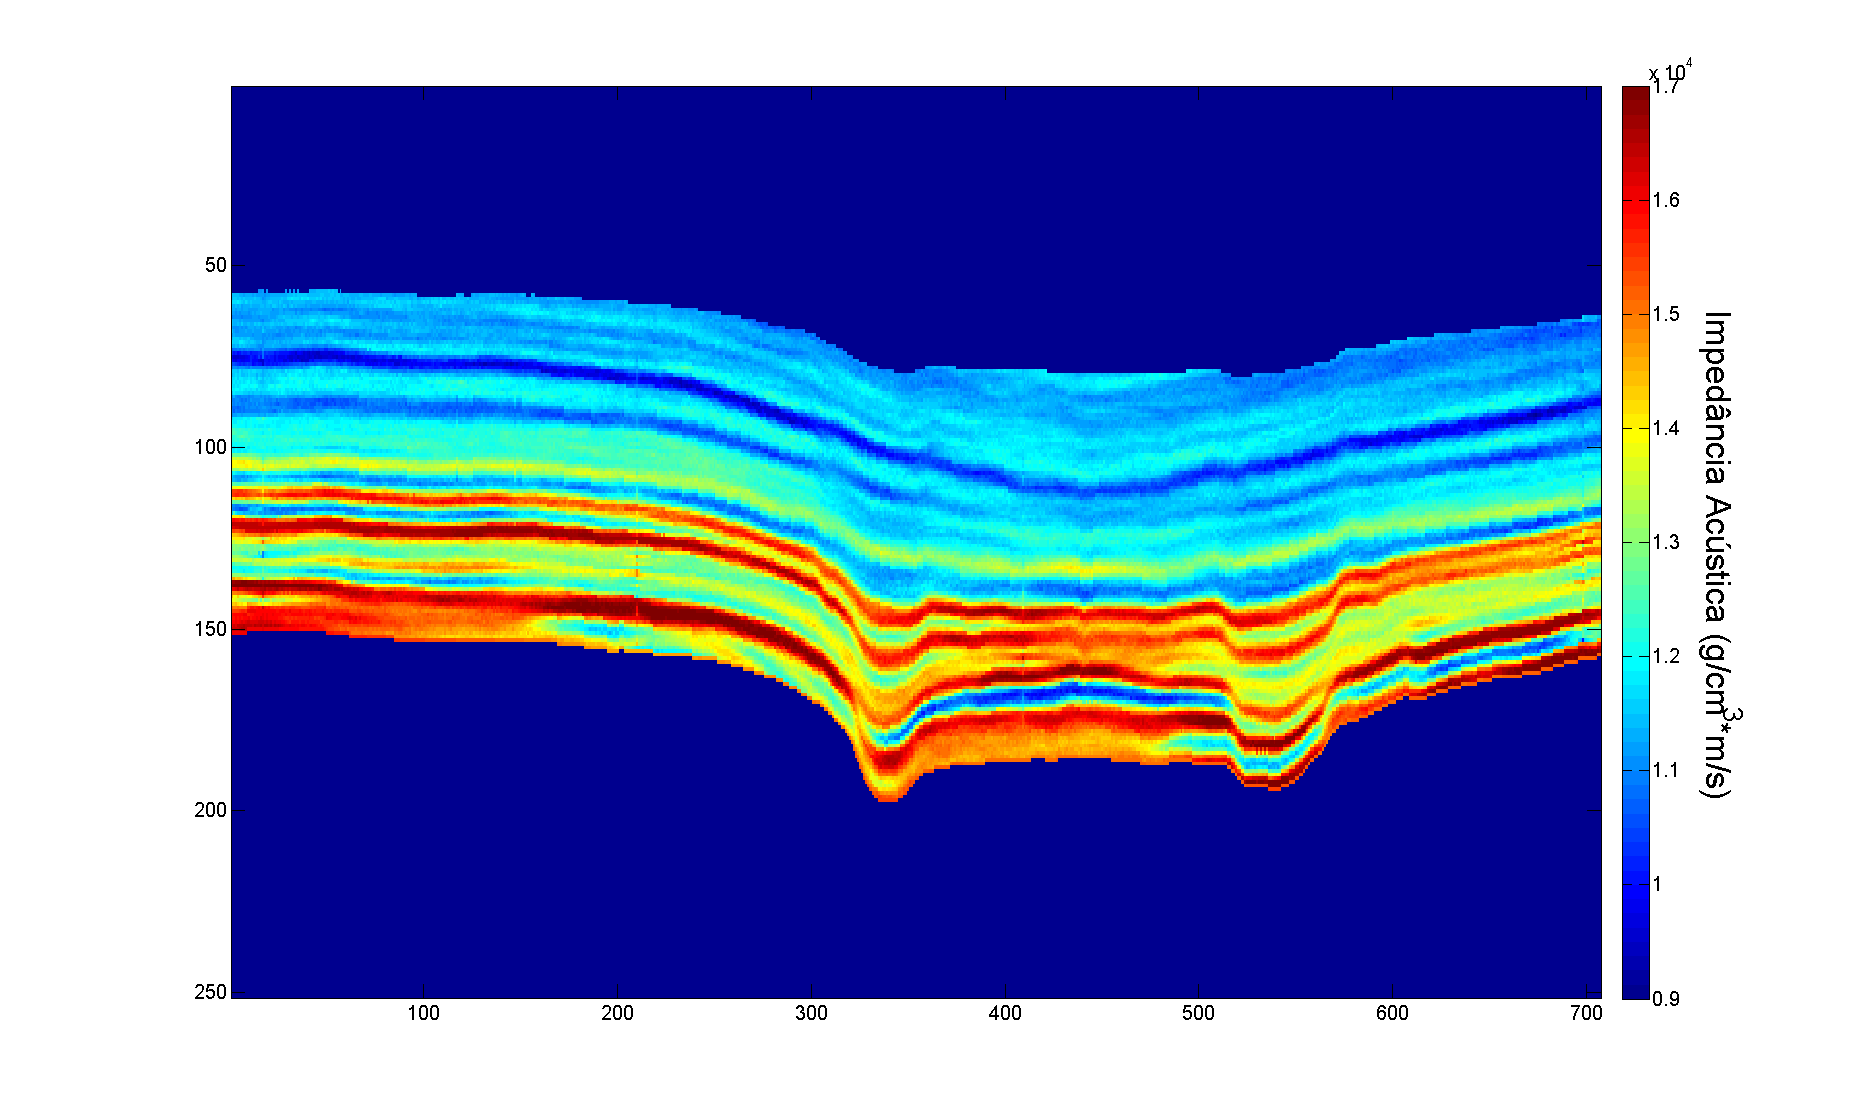
\includegraphics[width=\textwidth]{fig/mapdss1it-20realz-filt}
%   \caption{Média das amostras da SSD utilizando MAP como imagem
%   secundária}
%   \label{fig:mapDSS}
% \end{center}
% \end{figure}
% 
% 
% \begin{figure}[htp]
% \begin{center}
%   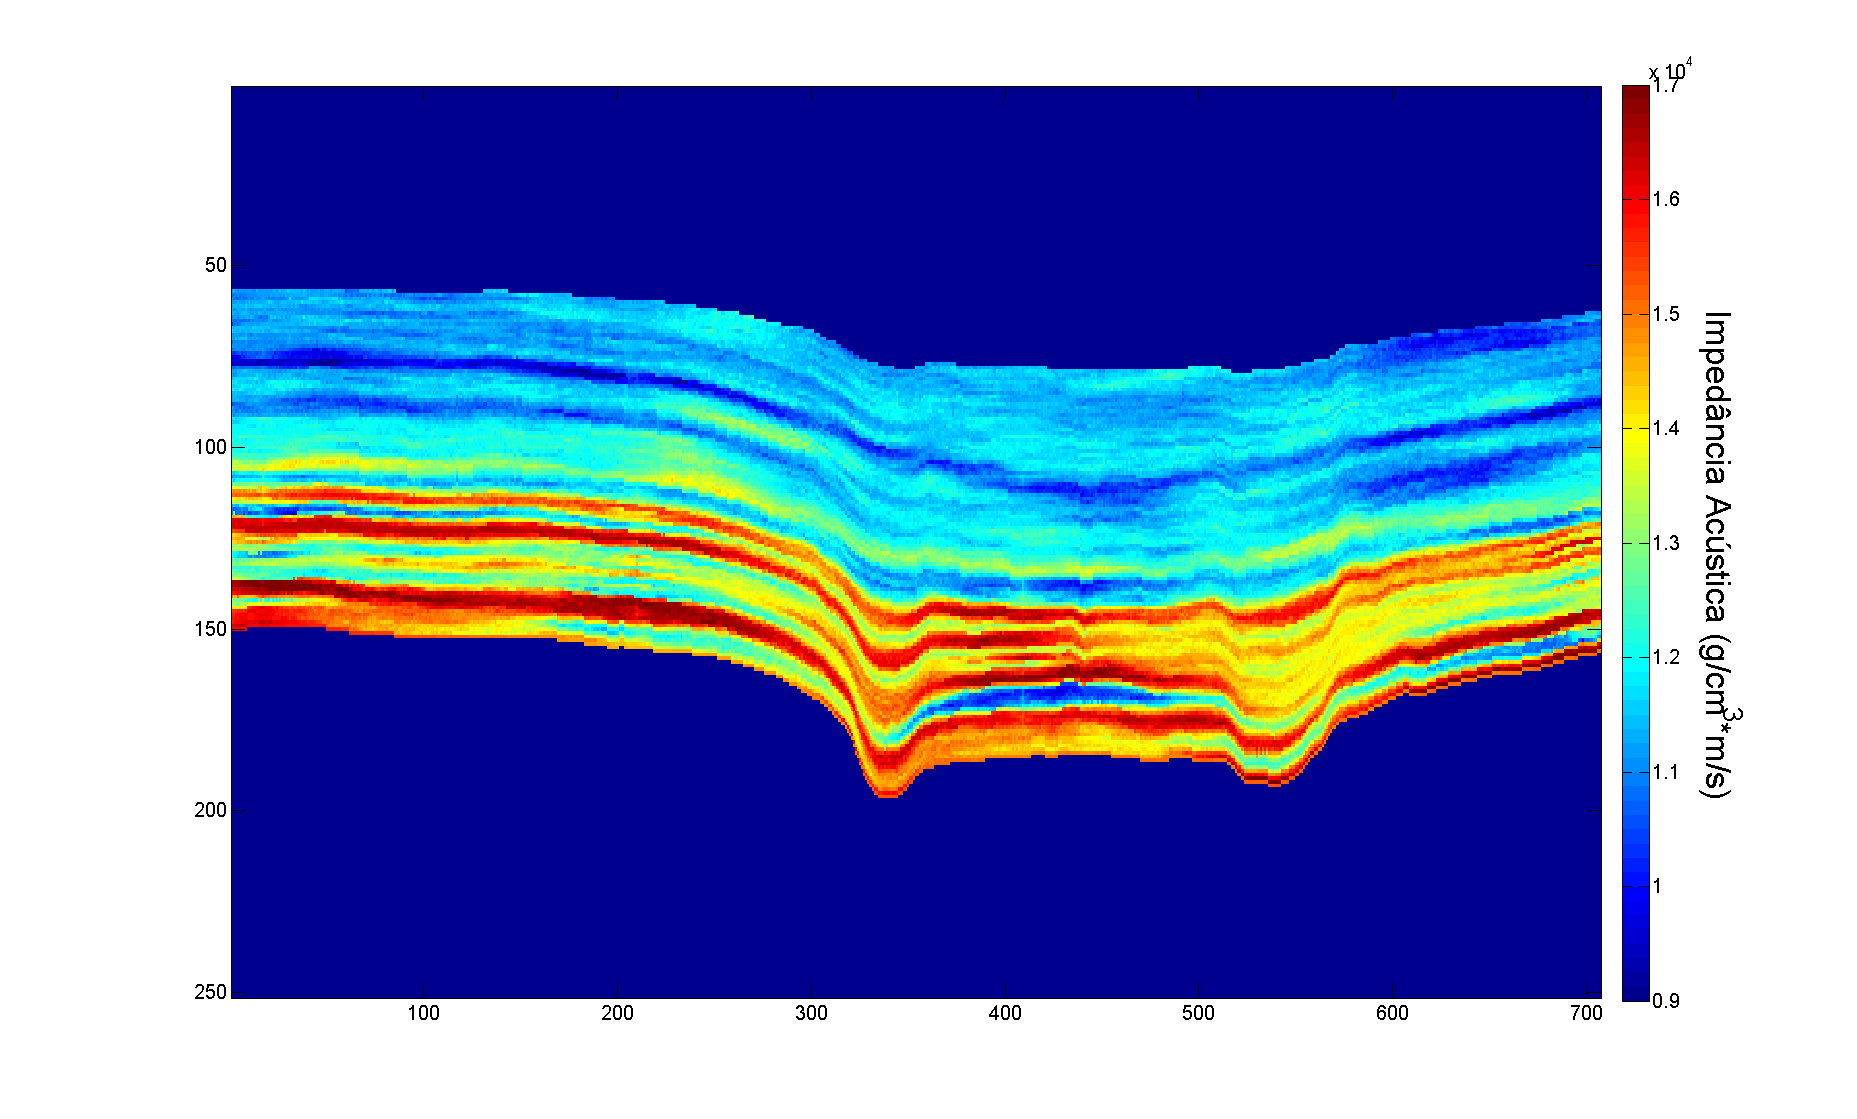
\includegraphics[width=\textwidth]{fig/dss10it-20realz}
%   \caption{Média das amostras após 10 iterações da GSI}
%   \label{fig:dss10result}
% \end{center}
% \end{figure}
% 
% A metodologia descrita na literatura para a GSI não aplica a filtragem dos dados
% para amostrar somente os resíduos, ou alta frequência. Utilizar o modelo de
% baixa frequência como informação \textit{a priori} foi identificado como uma
% regularização importante para agilizar a inversão e amostragem. Principalmente
% para a SSD, filtrar os dados resulta em uma distribuição global com menor
% variância, pois assumindo um modelo de baixa frequência são definidas médias
% locais e as amostras são geradas em torno desta média, respeitando a
% distribuição do poço filtrado. Sem a filtragem, a informação da média local não
% é utilizada, amostrando-se toda a distribuição original do poço em todos os
% pontos da região de interesse. A Figura \ref{fig:pocoFilteN} mostra a comparação
% dos histogramas dos dados filtrados e não filtrados. Portanto, utilizar o modelo
% de baixa frequência insere um viés no resultado e diminui a incerteza dada pela
% variância, mas a incerteza referente a escolha do modelo de baixa precisa ser
% levada em consideração.
% 
% 
% \begin{figure}
%         \centering
%         \begin{subfigure}[b]{0.45\textwidth}
%                 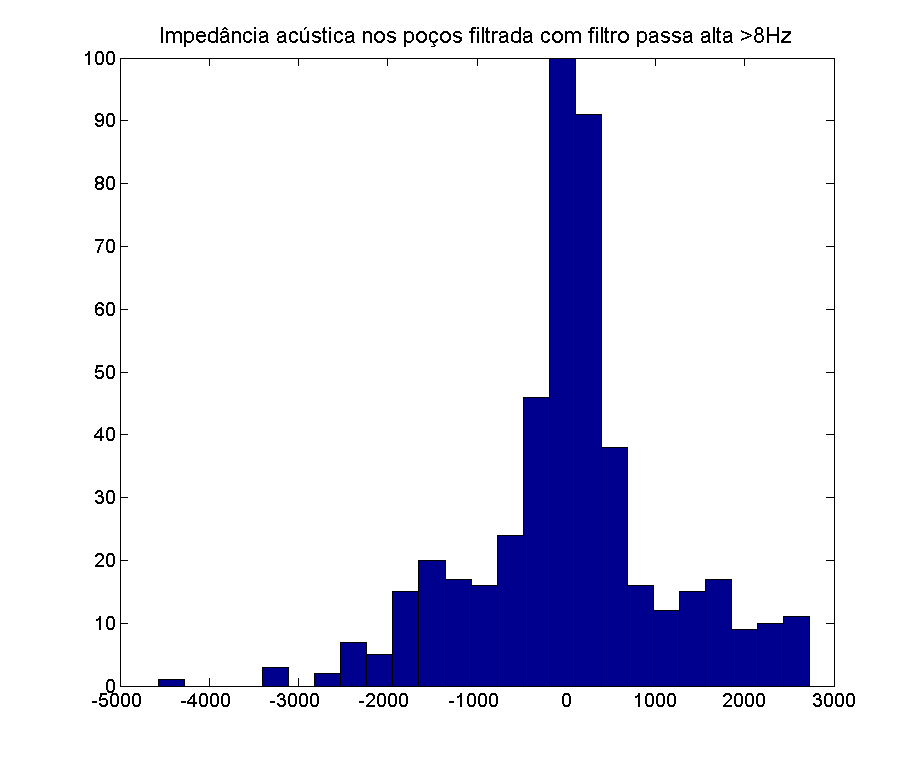
\includegraphics[width=\textwidth]{fig/IA_com_filtro}
%                 \caption{Dados filtrados}
%         \end{subfigure}%
%         \hfill
%         \begin{subfigure}[b]{0.45\textwidth}
%                 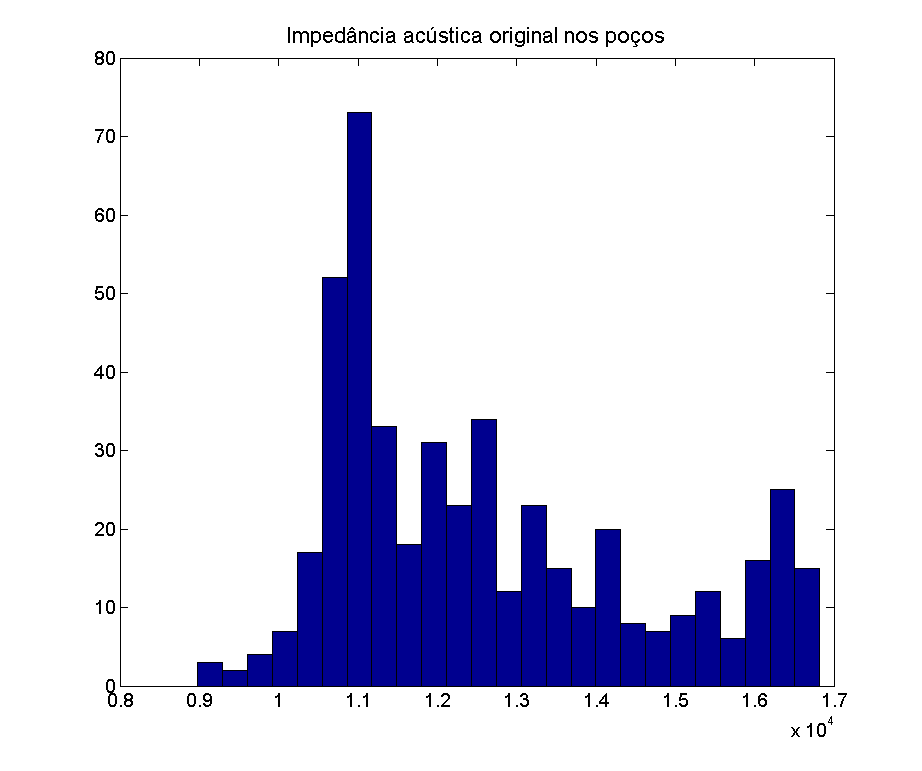
\includegraphics[width=\textwidth]{fig/IA_sem_filtro}
%                 \caption{Dados originais}
%         \end{subfigure}
%         \caption{Comparação dos dados de poços filtrados}\label{fig:pocoFilteN}
% \end{figure}
% 




\section{Proposta e Plano de Trabalho}

Os resultados preliminares apontam que é possível obter imagens de
inversão acústica em maior resolução. Entretanto, a aplicabilidade
do modelo depende da existência de conjunto de pares de imagens
de alta e baixa resolução para treinamento da rede e, consequentemente,
o limite da capacidade de inserção de altas frequências das imagens previstas
será limitada pelo faixa de altas frequências das imagens de treinamento.

Ao final da pesquisa se espera ter respostas para as seguintes questões:
\begin{itemize}
 \item o modelo de rede convolucional é capaz de aumentar a Resolução de imagens de impedância
quantitativamente?
 \item As imagens de teste apresentaram maior resolução que as imagens originais, sob o ponto 
de vista de altas frequências?
 \item Quais as faixas de alta frequências foram inseridas?
 \item Como as redes neurais aprenderam as altas frequências?
 \item É possível parametrizar o processo de super-resolução para imagens pós-inversão?
 \item Qual o limite de alta frequência é possível inserir nas imagens de alta resolução?
 \item Existe coerência geoestatística no resultado do modelo convolucional?
\end{itemize}

A proposta para o restante do projeto é implementar a rede convolucional para
realizar super-resolução sobre valores contínuos, realizar a análise de incerteza
sobre os resultados da rede convolucional, adaptar o modeo para realizar a super-resolução
de imagens em dimensões maiores e analisar o comportamento da rede para inversão
com um conjunto de dados reais.
Os resultados obtidos serão comparados com os resultados da GSI em
termos de variância e qualidade do resultado baseado na metodologia de
\cite{coleou_qualityanomalyinv}, amplamente utilizada para avaliação dos
resultados da inversão sísmica na indústria.
% 
% A metodologia de \cite{caers_distance_kernels_MDS} será integrada na proposta
% para possibilitar a análise da incerteza envolvida com os parâmetros e dados de
% entrada definidos pelo especialista, como o modelo de baixa, \textit{wavelets} e
% horizontes, pois a essas incertezas geológicas são apontadas como maiores
% influências na incerteza do resultado da inversão \citep[p.
% 133]{caers2011modeling}. Para tanto, será proposto um esquema de amostragem com
% Monte Carlo para selecionar os dados de entrada aleatoriamente a cada amostragem
% do resultado da inversão. Após obter várias amostras com combinações diferentes
% de dados de entrada, uma análise baseada em \textit{Multi-Dimensional Scaling}
% será aplicada para avaliar a sensibilidade ao variar cada parâmetro de entrada
% na incerteza final do resultado da inversão. Será utilizada como métrica as
% medidas de \textit{Quality-Anomaly} \citep{coleou_qualityanomalyinv}.
% 

O caráter de originalidade do trabalho é garantido pelas contribuições para a
aprendizado por redes neurais convolucionais e inversão sísmica.
A primeira contribuição está realcionada com o desenvolvimento de um
novo modelo de rede convolucional para super-resolução.
A segunda contribuição será modelar as incertezas presentes nos dados
de saída da rede para obter um entendimento sobre que tipo de modificação
as redes causam nas imagens e quais frequências são inseridas passaram a existir
nas imagens de alta resolução que não estavam presentes nas imagens de baixa resolução.

O caráter de ineditismo é garantido, pois não se verificou na literatura uma
abordagem de super-resolução para a inversão sísmica que permita um
ganho quantitativo e qualitativo das imagens da propriedade invertida.
Além disso, 

O caráter de não-trivialidade é obserado, pois a implementação da...

Dentre os periódicos que apresentam trabalhos relacionados com esta área, se
destacam os seguintes com suas classificações no Qualis para Ciências da
Computação:

\begin{itemize}
  \setlength{\itemsep}{0pt}
  \setlength{\parskip}{0pt}
  \item IEEE Trans. on Geoscience and Remote Sensing
  \item ISSN: 0196-2892 - IEEE - Qualis A1
\end{itemize}

\begin{itemize}
  \setlength{\itemsep}{0pt}
  \setlength{\parskip}{0pt}
  \item Journal of Computational Physics
  \item ISSN: 0021-9991 - Elsevier - Qualis A1
\end{itemize}

\begin{itemize}
  \setlength{\itemsep}{0pt}
  \setlength{\parskip}{0pt}
  \item Computers \& Geosciences
  \item ISSN: 0098-3004 - Elsevier - Qualis A2
\end{itemize}


\begin{itemize}
  \setlength{\itemsep}{0pt}
  \setlength{\parskip}{0pt}
  \item Computational Geosciences
  \item ISSN: 1420-0597 - Springer - Qualis B1
\end{itemize}


\begin{itemize}
  \setlength{\itemsep}{0pt}
  \setlength{\parskip}{0pt}
  \item Geophysics
  \item ISSN: 0016-8033 - Society of Exploration Geophysicists - Qualis A2 Interdisciplinar
\end{itemize}


\begin{itemize}
  \setlength{\itemsep}{0pt}
  \setlength{\parskip}{0pt}
  \item Mathematical Geosciences
  \item ISSN: 1874-8961 - Springer - Qualis A2 Interdisciplinar
\end{itemize}

